\documentclass[a4paper,12pt]{report}

\usepackage{alltt, fancyvrb, url}
\usepackage{graphicx}
\usepackage[utf8]{inputenc}
\usepackage{float}
\usepackage{hyperref}

% Questo commentalo se vuoi scrivere in inglese.
\usepackage[italian]{babel}

\usepackage[italian]{cleveref}

\title{Relazione \\``SMOL''}

\author{Ettore Farinelli \\ Marco Galeri ciao \\ Giovanni Paradisi \\ Mounir Samite}
\date{\today}


\begin{document}

\maketitle

\tableofcontents


%------------------------------ANALISI------------------------------
\chapter{Analisi}

%REQUISITI
\section{Requisiti}

Il software, commissionato dal gestore del centro di ricerca ``Aperture Laboratories Inc.''\footnote{\url{http://aperturescience.com/}}, mira alla costruzione di una intelligenza artificiale di nome GLaDOS (Genetic Lifeform and Disk Operating System).
%
Per intelligenza artificiale si intende un software in grado di assumere decisioni complesse in maniera semi autonoma sugli argomenti di sua competenza, a partire dai vincoli e dagli obiettivi datigli dall'utente.

\subsubsection{Requisiti funzionali}


\subsubsection{Requisiti non funzionali}

%ANALISI E MODELLO DEL DOMINIO
\section{Analisi e modello del dominio}


%------------------------------DESIGN------------------------------
\chapter{Design}

%ARCHITETTURA
\section{Architettura}

L'architettura di GLaDOS segue il pattern architetturale MVC.
%
Più nello specifico, a livello architetturale, si è scelto di utilizzare MVC in forma ``ECB'', ossia ``entity-control-boundary''\footnote{
Si fa presente che il pattern ECB effettivamente esiste in letteratura come ``istanza'' di MVC, e chi volesse può utilizzarlo come reificazione di MVC.
}.
%
GLaDOS implementa l'interfaccia AI, ed è il controller del sistema.
Essendo una intelligenza artificiale, è una classe attiva.
%
GLaDOS accetta la registrazione di Input ed Output, che fanno parte della ``view'' di MVC, e sono il ``boundary'' di ECB.
Gli Input rappresentano delle nuove informazioni che vengono fornite all'IA, ad esempio delle modifiche nel valore di un sensore, oppure un comando da parte dell'operatore.
Questi input infatti forniscono eventi.
Ottenere un evento è un'operazione bloccante: chi la esegue resta in attesa di un effettivo evento.
Di fatto, quindi, GLaDOS si configura come entità \textit{reattiva}.
Ogni volta che c'è un cambio alla situazione del soggetto, GLaDOS notifica i suoi Output,
informandoli su quale sia la situazione corrente.
%
Conseguentemente, GLaDOS è un ``observable'' per Output.

\begin{figure}[h]
\centering{}
%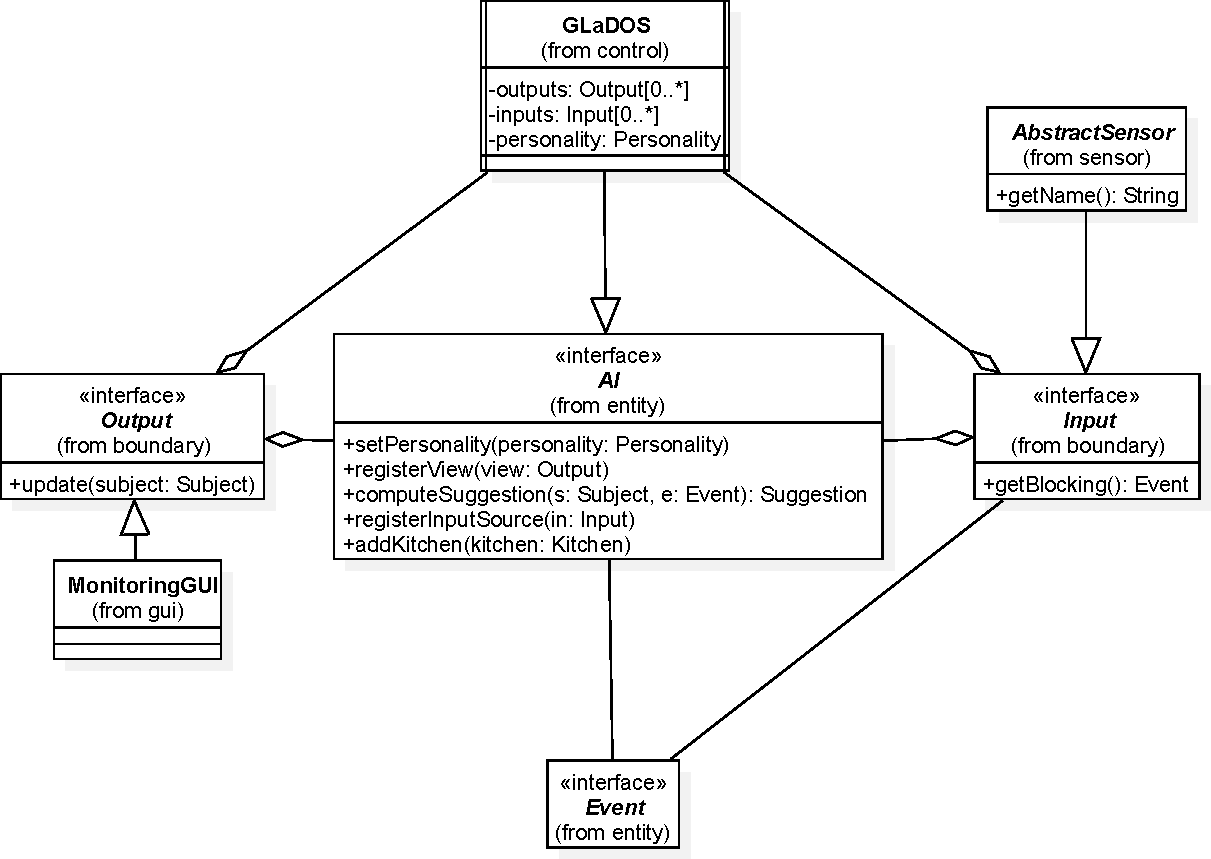
\includegraphics[width=\textwidth]{img/arch}
\caption{Schema UML architetturale di GLaDOS. L'interfaccia \texttt{GLaDOS} è il controller del sistema, mentre \texttt{Input} ed \texttt{Output} sono le interfacce che mappano la view (o, più correttamente in questo specifico esempio, il boundary). Un'eventuale interfaccia grafica interattiva dovrà implementarle entrambe.}
\label{img:goodarch}
\end{figure}

Con questa architettura, possono essere aggiunti un numero arbitrario di input ed output
all'intelligenza artificiale.
%
Ovviamente, mentre l'aggiunta di output è semplice e non richiede alcuna modifica all'IA, la
presenza di nuovi tipi di evento richiede invece in potenza aggiunte o rifiniture a GLaDOS.
%
Questo è dovuto al fatto che nuovi Input rappresentano di fatto nuovi elementi della business
logic, la cui alterazione od espansione inevitabilmente impatta il controller del progetto.

In \Cref{img:goodarch} è esemplificato il diagramma UML architetturale.

%DESIGN DETTAGLIATO
\section{Design dettagliato}

\subsection*{Ettore Farinelli}
roba di Ettore
\subsection*{Marco Galeri}
roba di Marco
\subsection*{Giovanni Paradisi}
roba di Giovanni
\subsection*{Mounir Samite}
roba di Mounir


%------------------------------SVILUPPO------------------------------
\chapter{Sviluppo}

%TESTING
\section{Testing automatizzato}

%METODOLOGIA_DI_LAVORO
\section{Metodologia di lavoro}
un po di roba sul DVCS

\subsection*{Ettore Farinelli}
roba di Ettore
\subsection*{Marco Galeri}
roba di Marco
\subsection*{Giovanni Paradisi}
roba di Giovanni
\subsection*{Mounir Samite}
roba di Mounir

%NOTE_DI_SVILUPPO
\section{Note di sviluppo}

\subsection*{Ettore Farinelli}
roba di Ettore
\subsection*{Marco Galeri}
roba di Marco
\subsection*{Giovanni Paradisi}
roba di Giovanni
\subsection*{Mounir Samite}
roba di Mounir

%------------------------------COMMENTI_FINALI------------------------------
\chapter{Commenti finali}

un po de roba

%AUTOVALUTAZIONE_E_LAVORI_FUTURI
\section{Autovalutazione e lavori futuri}
\subsection*{Ettore Farinelli}
roba di Ettore
\subsection*{Marco Galeri}
roba di Marco
\subsection*{Giovanni Paradisi}
roba di Giovanni
\subsection*{Mounir Samite}
roba di Mounir

%DIFFICOLTA(OPZIONALE)
\section{Difficoltà incontrate e commenti per i docenti}

\textbf{opzionale}


\appendix

%------------------------------GUIDA------------------------------
\chapter{Guida utente}



\bibliographystyle{alpha}
\bibliography{report}

\end{document}
